\documentclass{homework}
% \usepackage{graphicx} % Required for inserting images
\usepackage{amsmath}
\usepackage{gensymb}
\usepackage{subfig}
\usepackage{float}

\class{ECEN 5407}
\title{Homework 3}
\author{Sean Jennings}
\date{October 11, 2023}

\begin{document}
\maketitle

\section{Problem 1}
\begin{letterenum}
\item Figure \ref{fig:solar-circuit} shows the equivalent circuit of a single
solar cell. Table \ref{table:solar-parameters} summarizes the parameters 
\begin{center}
    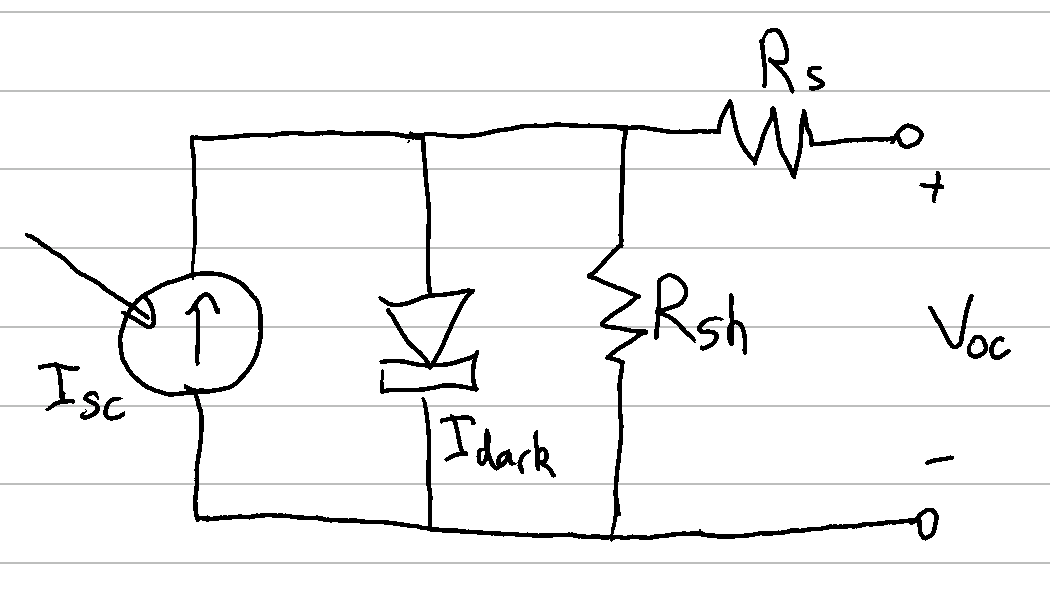
\includegraphics[width=0.5\linewidth]{Images/solar_circuit.png}
    \captionof{figure}{Solar Cell Equivalent Circuit}
    \label{fig:solar-circuit}
\end{center}
\begin{center}
    \begin{tabular}{| c | c |}
        \hline
        Symbol & Description \\
        \hline
        $I_{sc}$ & Short-circuit current \\
        $I_{dark}$ & "Dark" current \\
        $R_{sh}$ & Shunt resistance \\
        $R_s$ & Series resistance \\
        $V_{oc}$ & Open-circuit Voltage \\
        \hline
    \end{tabular}
    \captionof{table}{Solar Cell Cicruit Parameters}
    \label{table:solar-parameters}
\end{center}

The photovoltaic effect of incident light on the cell can be modeled as a current
source. The current that flows when the cell's terminals are connected without
a load is the "short-circuit current". Once a load is placed across the terminals
a voltage develops and causes a certain amount of the generated current,
know as "dark current," to flow through the device, without reaching the load.
The name "dark current" refers to the fact that a current will flow across
the cell, even in the dark, if a voltage, $V > 0$, is applied across the terminals.
Since current does not flow when voltage polarity is reversed, $V < 0$, it is
modeled as a diode.  \cite{nelson_physics_2003}

The "series resistance" refers to the voltage potential/heat that is dissipated
due to the material within the cell through which the current flows as well
as electrical contacts. The "shunt resistance" refers to the current that is lost
through leakage. This is common in poorly rectifying devices. (Rectifying action
refers to the asymmetrical material property that forms a "barrier" which drives
electric charge through the circuit, e.g. the p-n junction in semiconductors.)

The open-circuit voltage is the voltage which is reached when the terminals of
the cell are open (i.e. all the current flows through as dark or shunt current).

If the cell were ideal, then the series resistance would be short-circuit, and
the shunt resistance open, i.e. $R_s = 0$ and $R_{sh} = \infty$. The dark current
is present even in the ideal case, since it is inseparable from the rectifying
behavior that allows current to flow at all.

\item The diode current is given by the following:
\begin{equation*}
    I_{dark} = I_0 (e^{qV / k_B T} - 1)
    \label{eq:dark-current}
\end{equation*}
where $I_0$ is a constant dependent on the material and temperature, $q$ is the
charge of an electron, $V$ is the voltage across the cell, $k_B$ is Boltmann's
constant, and $T$ is the temperature.

\item By Kirchoff's current law, the current that flows across the terminals of
the cell is the sum of current entering and leaving the top-most node of the circuit
\begin{equation}
    I = I_{sc} - I_{dark} - I_{sh}
    \label{eq:current-sum}
\end{equation}
where $I$ is the output current, $I_{sh}$ is the current flowing across the shunt.
The voltage at the upper most node is related to the terminal voltage by:
\begin{equation}
    V_{upper} = V + R_s I
    \label{eq:voltage-drop}
\end{equation}
since the series resistance causes a voltage drop proportional to current.
Applying Ohm's law and combining equations (\ref{eq:dark-current}),
(\ref{eq:current-sum}), and (\ref{eq:voltage-drop}) characteristic
equation including parasitic losses:
\begin{equation*}
    I = I_{sc} - I_0 (e^{q (V + R_s I)/ k_B T} - 1) - \frac{V + R_sI}{R_{sh}}
    \label{eq:solar-characteristic}
\end{equation*}

\item The short-circuit current is related to the incident spectral
photon flux density, $b_s(E)$, and the material's quantum efficiency, $QE(E)$,
by the following equation
\begin{equation*}
    I_{sc} = q \int_{0}^{\infty} b_s(E) QE(E) dE A
\end{equation*}
$QE(E)$ is the material-dependent probability that a incoming photon
of a particular energy will cause an electron to flow through the circuit.
$b_s(E)$ is the number of photons in a given energy band that enter a
unit area per unit time. $A$ is the area of the cell, and $q$ is again
the charge of an electron.

\item The open-circuit voltage $V_{oc}$ can be derived from equation
(\ref{eq:solar-characteristic}), with the simplying assumptions of
no parasitic losses ($R_s=0$, $R_{sh}=\infty$). Since in a open circuit
$I=0$, the open-circuit voltage is when dark current and short-circuit
current are equal
\begin{equation*}
    V_{oc} = \frac{k_BT}{q}\ln(\frac{I_{sc}}{I_0} + 1)
\end{equation*}


\item At open-circuit $V=0$ and in short-circuit $I=0$, so in either 
case the power output is zero: $P=VI=0$. Figure (\ref{fig:iv-curve}) shows the
I-V curve.

\begin{center}
    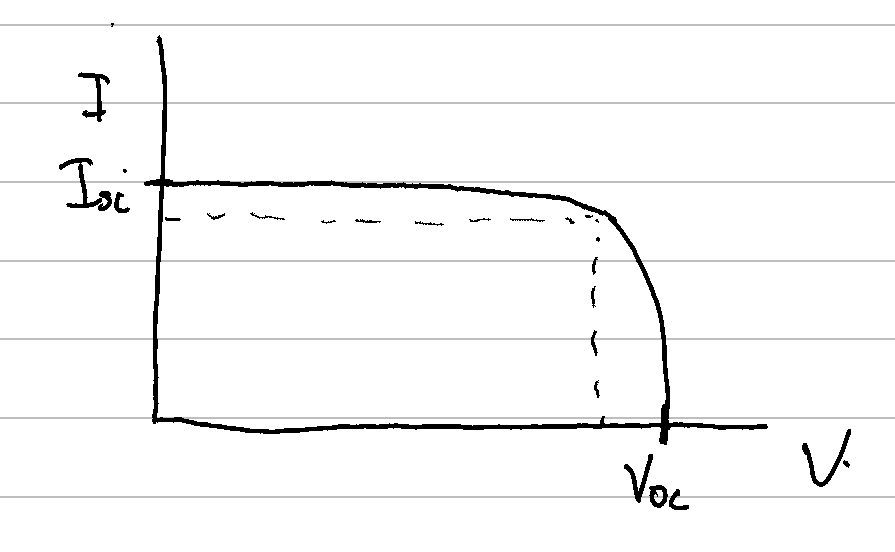
\includegraphics[width=0.5\linewidth]{Images/iv_curve.png}
    \captionof{figure}{IV Curve}
    \label{fig:iv-curve}
\end{center}

\item Increased solar irradiance will increase the value of $b_s(E)$ across
the light spectrum, therefore increasing the short-circuit current $I_{sc}$.
Since for a given $V$ (and neglecting parasitic losses),
the dark current is constant, the output current will therefore also increase.
However, in practice, higher irradiance leads to higher temperatures which
increases the series resistance. Above a certain optimal point, increased
irradiance causes resistance to increase faster than short-circuit current.

A change in temperature has counteracting effects on the physics of the
p-n junction. On one hand, the electron band gap is reduced, causing
an increase in short circuit current $I_{sc}$. However, the dark current
also increases so that the open-circuit voltage $V_{oc}$ also decreases.
The increase in dark current outweighs the increase in short circuit current,
thus reducing the overall power output.

\item The maximum operating point is defined in terms of power output. The
maximum power point (MPP) occurs at some point slightly less than $V_{oc}$,
before the current begins to rapidly drop to 0. Various MPP tracking (MPPT)
control algorithms can be implemented to control the operating voltage of the PV
cell to follow the maximum, but "Perturb and Observe" is the most commonly
implemented due to its ease of implementation.

It works by slightly "perturbing" the operating voltage and "observing" the
change in power. If the power increases, it will continue to change the
voltage in that direction, otherwise it will change the voltage in the
opposite direction. 
\end{letterenum}

\section{Problem 2}
\begin{letterenum}
\item It seems to be pretty standard for manufacturers to provide:
\begin{itemize}
    \item maximum power output,
    \item voltage at maximum power,
    \item current at maximum power,
    \item open-circuit voltage, and
    \item short-circuit current
\end{itemize}
across two standardized operating conditions: standard test conditions
(STC, 25$\degree$C and 1000 W/m$^2$ irradiance) and nominal operating conditions
(40$\degree$C and 800 W/m$^2$). They also provide
\begin{itemize}
    \item temperature coeficients for how voltage, current, and power vary
        as a (linear) function of temperature.
    \item maximum power efficiency
    \item various electric design parameters (e.g. maximum system voltage, maximum
        fuse rating), as well as
    \item mechanical design parameters (weight, dimensions, etc.).
\end{itemize}

\item For 6 cells connected in series, total current through all cells $I_{total}$ is equal
    to the current through each cell, i.e. $I_{total} = I_{cell}$. The total
    voltage drop is the sum of the voltage drops: $V_{total} = 6 V_{cell}$.
\item For 6 cells in parallel, total voltage is the cell voltage: $V_{total} = V_{cell}$.
    Total current is the sum: $I_{total} = 6 I_{cell}$.
\item Assuming that there is some MPPT algorithm running, then the voltage and current
    will both be decreased in order to maintain maximum power. As a result, both
    will be some fraction of the previous value: $V_{cell,new} = p V_{cell}$ and
    $I_{cell,new} = r I_{cell}$, where $0 < p,r < 1$. In either module setup, 
    the total voltage and current will be scaled the same $p$ and $r$, respectively.
    For example, for the series setup:
    \begin{align*}
        V_{total,new} &= 6 V_{cell,new} = 6 p V_{cell} = p V_{total} \\
        I_{total,new} &= V_{cell,new} = r V_{cell} = r V_{total} \\
    \end{align*}
\end{letterenum}

\section{Problem 3}

\begin{letterenum}
\item We assume that 80\% ($\rho = 80$) of the graviational potential energy
    (per unit time) is converted to power. Then, we have the relation:
    \begin{equation*}
        P = \rho \frac{dE}{dt} = \rho \frac{d}{dt}(mgh) = \rho \dot{m}gh
    \end{equation*}
    where $P$ is the power generated, $\frac{dE}{dt}$ is the rate of change
    of energy over time. $m$ is the mass, $\dot{m}$ is mass flow rate, $g=9.81m/s^2$
    the force of gravity and $h$ is the hydraulic head.

    Including unit conversion, we find:
    \begin{equation*}
        P = 0.8 (396259 \text{ gal/sec}) (0.00379 m^3/gal)
            (9.81 \text{ m/s}^2) (590 \text{ ft} * 0.3048 \text{ m/ft})
            = 2.120 \text{ MW}
    \end{equation*}

\item In terms of energy conversion, run-of-river plants do not have an
    resevoir and so are not dispatchable. Also, since run-of-river plants
    are typically smaller in size. There would be a different
    type of turbine used, which would effect the efficiency of conversion:
    typically Pelton wheels are used for lower power output, versus
    Francis turbines for large dams.
\item Some of the advantages of hydro are that:
\begin{enumerate}
    \item in places which have the resource, it can generate huge amounts
        of power (many of the largest power plants in the world are hydro),
    \item it has zero carbon emissions, and
    \item it is (to some degree) dispatchable (i.e. for dammed hydro).
\end{enumerate}
There's a number of disadvantages as well:
\begin{enumerate}
    \item It is geographically constrained (the location needs to have
        water and a height difference such as mountains),
    \item there are ecological concerns over the displacement of natural
        environments,
    \item it is variable depending on the season and water year, and
    \item it has many other priorities other than power generation (this can
        lower capacity factor and dispatchability).
\end{enumerate}
Probably the largest reason it is not currently begin expanded in the US
is that we have already developed most of the locations which contain
significant power potential. 

\end{letterenum}

\section{Problem 4}
\begin{letterenum}
    \item The turn ratio is $\alpha = 440 / 48 = 9.1667$, so the output is
        $V_2 = V_1 / \alpha = 110 \V / (440 / 48) = 12 \V$ (rms).
    \item The turns ratio is 1:2. The secondary has more coils so it is
    the high side. Thus, peak to peak voltage across the 
    second coil is $V_{2,pp} = 170 \V * 2 = 340 \V$. The RMS is given by
    $V_{2,rms} = V_{2,pp}/\sqrt{2} = \boxed{240.4 \V}$. And the expression
    as a function of time is:
    \begin{equation*}
        v_2(t) = 340 \cdot \cos(60 * 2\pi t)  \Vb
    \end{equation*}
    This would be a typical waveform in the US since US uses 60Hz, whereas
    Europe uses 50Hz.

    \item The turns ratio is 10:1 so the input current is $150$ mA$/10 = 15$ mA.

    The input power is then: $P = VI = 120 \V \cdot 150$ mA $= 1.8$ W.

    This is an unreasonably small power output for a small appliance. For
    example, a typical toaster consumes ~1000W, while an LED light bulb 
    consumes about 10W.
\end{letterenum}

\section{Problem 5}

\begin{letterenum}
\item This is a step-up transformer and is used to step up the voltage
    from levels appropriate for the generators based on their physics,
    to a higher level appropriate for transmission.
\item More efficiency is achieved at higher transmission voltages since
    the real power losses in transmission line are $P = VI = RI^2$ (using
    power definition and Ohm's law). Thus, transmission losses scale with the
    square of current. For a constant power output, a higher voltage means
    a reduced current, which in turn reduces the power losses quadratically.
\item The new secondary coils to old secondary coils ratio is $765/345 = 2.217$.
    So there are 2.217 times more coils after the replacement.
\item For a constant power output, the current reduced by the same coils factor,
    so the ratio from new current to old is $1/2.217 = 0.451$.
\item Since power losses are proportional to $I^2$, the ratio of new power loss
    to old is $0.451^2 = 20.34\%$.
\end{letterenum}



\bibliography{RenEngHW3}

\end{document}
